\documentclass[conference]{IEEEtran}
\IEEEoverridecommandlockouts
% The preceding line is only needed to identify funding in the first footnote. If that is unneeded, please comment it out.
\usepackage{cite}
\usepackage{amsmath,amssymb,amsfonts}
\usepackage{algorithmic}
\usepackage{graphicx}
\usepackage{textcomp}
\usepackage{xcolor}
\usepackage[hidelinks]{hyperref}
\def\BibTeX{{\rm B\kern-.05em{\sc i\kern-.025em b}\kern-.08em
    T\kern-.1667em\lower.7ex\hbox{E}\kern-.125emX}}
\begin{document}

\title{Road Accident Prediction in Time and Space}

\author{\IEEEauthorblockN{1\textsuperscript{st} Antoine Hébert}
\IEEEauthorblockA{\textit{Department of Computer Science and Software Engineering} \\
\textit{Concordia University}\\
Montréal, Québec, Canada \\
an\_heb@encs.concordia.ca}
\and
\IEEEauthorblockN{1\textsuperscript{st} Timothée Guédon}
\IEEEauthorblockA{\textit{Department of Computer Science and Software Engineering} \\
\textit{Concordia University}\\
Montréal, Québec, Canada \\
t\_guedon@encs.concordia.ca}
\and
\IEEEauthorblockN{3\textsuperscript{rd} Tristan Glatard}
\IEEEauthorblockA{\textit{Department of Computer Science and Software Engineering} \\
\textit{Concordia University}\\
Montréal, Québec, Canada \\
tglatard@encs.concordia.ca}
\and
\IEEEauthorblockN{4\textsuperscript{th} Brigitte Jaumard}
\IEEEauthorblockA{\textit{Department of Computer Science and Software Engineering} \\
\textit{Concordia University}\\
Montréal, Québec, Canada \\
bjaumard@cse.concordia.ca}}

\maketitle

\begin{abstract}
Road accidents are an important issue of our modern societies, responsible for millions of deaths and injuries. In this paper we show how one can leverage open datasets from a city like Montreal, Canada, to create some accident prediction models, using state-of-the-art big data analytics methods in Python. Such models could then be used in the context of road accident prevention, but also to identify key factors that can lead to a road accident, and eventually, help to elaborate new policies. This study also explains how we dealt with the severe class imbalance issue of the accident prediction problem, a recurrent issue that touches many other scientific domains like medical diagnoses or fraud detection. In particular, we show how we implemented Balanced Random Forests, a variant of the Random Forests machine learning algorithm, into the Scala and Python APIs of Apache Spark big data framework.

\end{abstract}

\begin{IEEEkeywords}
machine learning, road accidents prediction
\end{IEEEkeywords}

\section{Introduction}
\subsection{Context}
According to the World report on road traffic injury prevention, 2004, more than one million people die every year from car accidents and dozens of millions of people are being injured\cite{Peden2004}. In this report, the World Health Organization also describe road traffic systems as “the most complex and the most dangerous system with which people have to deal every day”. This issue is all the more important that the number of accidents is forecast to continue rising. In the last decade, Big Data Analytics has been emerging \cite{Gandomi2015}, allowing scientists to handle a very large amount of data, but also complex and heterogeneous data, in order to extract useful insights from it. In the context of accident prediction, Big Data Analytics could provide insights on the conditions leading to an increased risk of road accidents that could then be used to develop traffic-related policies and prevention operations. Our contributions include: 
\begin{itemize}
\item a demonstration of how simple and easily available datasets can be assembled to obtain meaningful features for road accident prediction,
\item a comparison of three different machine learning algorithm dealing with data imbalance in the context of road accident prediction,
\item the implementation of Balanced Random Forest introduced by Chen et al.\cite{Chen2004} in Apache Spark for efficient distributed training. 
\end{itemize}
All the source code used is publicly available on Github under the MIT license.\footnote{https://github.com/GTimothee/accident-prediction-montreal}

need to be extended:
  how our dataset is bigger because 6 years and precise because road segments


\subsection{Related work}
Accident prediction has been extensively studied in the last decade. Historically, variation of the Poisson regression such as the negative binomial regression were used to predict the number of accident which occurred on a given road segment. The features usually used include feature from the road such as the number of lanes, the average daily traffic, and the curvature, and weather features such as average precipitation and the temperature. In 2005, Chang \cite{Change2005} compared the performances of a negative binomial regression with that of an Artificial Neural Network to predict the number of accident during a year on a road segment from a major freeway in Taiwan. The dataset used contains data from the years 1997 and 1998, which resulted in 1338 accidents. The ANN achieved slightly better result, with an accuracy of 61.4\% on the test dataset. On the same dataset, Chang et al.\cite{Chang2005b} also used decision trees for accident prediction in order to get more insight on the important variable for accident prediction. It appears that the average daily traffic and the number of days with precipitation are the most useful features. The decision tree reached an accuracy of 52.6\% on the test dataset. Lin et al. \cite{Lin2015} compared Frequent Pattern trees and random forests for feature selection and then k nearest neighbor and bayesian network for real-time accident prediction. Using the mean and sometimes the standard deviation of time series corresponding to the weather condition, the visibility, the traffic volume, the traffc speed and the occupancy, their models predict the occurence of an accident at the end of the time series. They obtain the best result using the Frequent Pattern trees feature selection and the  (add accuracy)
We note that the used a small sample of the possible negative examples.

  In addition, some other work aim at predicting the serverity of an accident using various information from the accident in order to understand what causes an accident to be fatal. Chong et al. \cite{Chong2005} used decision trees, neural network and an hybrid model using a decision tree and a neural network. They obtained thes best performances with the hybrid model which reached an accuracy of 90\% for the prediction of fatal injuries. They identified that the seatbelt usage, the light conditions and the alcohol usage of the driver are the most important features.
 
To be continued.
To cite: \cite{Theofilatos2017, Abellan2013, Lin2015}

Recently, the outstanding progress of deep learning algorithms has resulted in their extensive use in every field, including in Geospatial machine learning (Convolutional Neural Network and Long Short-Term Memory neural network for example) \cite{Yuan2018, QChen2016}.





\section{Methods}
\subsection{Choosing a Big Data framework: Apache Spark or Dask}
According to Dask’s official website, “Dask is a flexible library for parallel computing in Python” \cite{dask}. Apache Spark, on the other hand, describes itself as “a fast and general-purpose cluster computing system” \cite{spark}. Both of them are accepted tools with wide supporting community, even though Apache Spark is a bigger and older project. Although we almost exclusively used Apache Spark’s Python API (called “pySpark”) in this study, we started our experiment using Dask. Some advantages of Dask over Spark made us chose it for our analysis in the first place; For example, Dask “is developed in coordination with […] projects like Numpy, Pandas and Scikit-Learn” \cite{dask}, all widely used Python packages in machine-learning and data science. It is also admitted that Dask is lighter than Spark and designed to be more flexible in terms of applications and algorithms. However, we found ourselves writing a lot more code using Dask than Spark for the same result. Spark map-reduce-based interface is very handy and allows easier processing of datasets. For all these reasons we found out that Spark fitted our needs best and we switched to it at an early time of the study.

\subsection{Algorithms selected}
For this study, we chose to focus on tree-based algorithms because they have proven their efficiency compared to classical statistical methods and allow for easier interpretability than deep learning algorithms. In particular, we implemented the Balanced Random Forests (BRF) algorithm in Apache Spark to deal with class imbalance which is a prominent issue in road accident prediction. To validate the performance of our version, we run an experiment with a simple synthetic dataset to compare its performances with the standard implementation of Random Forest (RF) in Spark using random under-sampling of the majority class. As expected, Balanced Random Forest performed better. Balanced Random Forests in one of the two methods proposed by Chen, Liaw, and Breiman\cite{Chen2004} to deal with class imbalance when using Random Forest. Balanced Random Forests are like Random Forests, but with a difference during the bootstrapping phase, for each tree of the forest, a random under-sampling of the majority class is performed in order to obtain a balanced sample. Intuitively, Balance Random Forest is an adaptation of random undersampling of the majority class making use of the fact that Random Forests are an ensemble method. Random undersampling usually performs better than more advanced methods like SMOTE or NearMiss \cite{Branco2016}. Chen, Liaw and Breiman\cite{Chen2004} also proposed in the same paper, the Weighted Random Forest (WRF) which consists in giving more weight to the minority class at the building time of each tree and during the measure of the gain in impurity and during the class prediction of each terminal node. While neither method is clearly better than the other in terms of prediction power, we chose BRF because it is found to be more computationally efficient (because of the under-sampling). Interestingly, Wallace et al. \cite{Wallace2011} presents a theoretical analysis of the data imbalance problem and suggest to use methods like Balance Random Forest. 
	
We decided to compare the performance of the Balanced Random Forests algorithm with the performances of one of the very efficient implementations of Gradient Boosted Trees: XGBoost which offers parameters to deal with data imbalance as well.

\subsection{Datasets}
We used three public datasets provided by the city of Montreal and the government of Canada: 
\begin{itemize}
\item Montreal Vehicle Collision: This dataset provided by the city of Montreal contains all the road collisions reported by the police in Montreal from 2012 to 2018. For each accident, the dataset contains the date and localization of the accident, information on the number of injuries and death, the number of vehicles involved, and information on the road condition. We used only the localization and the date of the accident since we do not have the other piece of information when no accident happened. Another dataset with all vehicle collision in Canada is available but without the localization of the accident, therefore we restrained our analysis to the city of Montreal.
\item National Road Network: This dataset provided by the government of Canada contains the geometry of all roads in Canada. For each road segment, a few meta-data are given. For roads in Quebec, the speed limit and the surface type are not provided. The data was available in various format, we chose to use the Keyhole Markup Language, which is a standard of the Open Geospatial Consortium since 2008. This format is based on the Extensible Markup Language (XML), which make it easier to read using existing implementation of XML parsers. 
\item Data Historical Climate Data: This dataset provided by the government of Canada contains hourly weather information measured at different weather stations across Canada. For each station and every hour, the dataset provides the temperature, the humidity, the wind direction and speed, the visibility, the atmospheric pressure and observations of atmospheric phenomenon such as snow, fog, rain, etc.
\end{itemize}

\subsection{Positive and negative examples generation}
This machine learning problem can be stated as a binary classification problem, the positive class is the occurrence of an accident and the negative class is the non-occurrence of an accident on a given road at a given date and hour. The vehicle collision dataset contains 150 thousands of collisions, among them $134 489$ contain the date, the hour and the localization of the accident. For each of these accidents, we identify the closest road segment. These pairs of a time and a road segment are used as positive examples. For the negative examples, we generated a random sample of 2 millions combinations of time and road segment which did not appear in the collision dataset.  The generation of these examples together with the join operation with the data from the other datasets made our dataset generation heavy. It resulted in an impractical amount of time and memory space requirements to generate the dataset. Our first implementation was querying the Historical Climate Data API in real-time with a cache mechanism. Our idea was to collect only the weather stations and hours necessary for our sample of negative examples, but it resulted in bad performances. We got a performance increase by first building a Spark data frame with all the Historical Climate Data for weather stations around Montreal and then joining the two datasets. We conducted a detailed analysis of our algorithm to improve its performances. We notably obtained a good performance increase by not persisting intermediary results of the road segment identification for accidents. As opposed to what we initially thought, recomputing these results was faster than writing and reading them in the cache. Finally, the identification of the road segment corresponding to accidents was very memory intensive, we modified this step to be executed by batch of one month.  With these improvements and a few other tricks including partitioning the data frame at key points in our algorithm, we managed to reduce the processing time to a reasonable time. We also used a cluster from “Compute Canada” to take maximum advantage of Apache Spark distributed nature for the generation of examples and the hyper-parameter tuning of our models.

\subsection{Feature Engineering}
Once we had our pairs of an hour and a road segment for positive and negative examples, we created features from this information. We created three types of features, weather features, features from the road segment and features from the date and time.

For the weather features, we used data from the Historical Climate Dataset. In order to estimate the weather information at the position of the road segment, we use the mean of the weather information from all the surrounding weather stations at the date and hour of the example weighted by the inverse of the square of the distance between the station and the road segment. We initially used the inverse of the distance, but we obtained a small improvement in performances when squaring the inverse of the distance. It makes sense since the weather information is probably much closer to the closest stations than the other ones. We tried higher power, but the results were not as good. It could be interesting to experiment with different power values for each weather information. We used all the weather information provided by the Historical Climate Dataset. The features are: the temperature, the dew point temperature which is a measure of the humidity, the real humidity percentage, the wind direction, the wind speed, the visibility, the atmospheric pressure, the Hmdx index, which is a measure of felt temperature and the wind chill which is another measure of the felt temperature using the wind information. In addition, the historical weather dataset, provide a multi-label categorical variable providing the observations of atmospheric phenomenon such as snow, fog, rain, etc. We used this last variable to create a binary variable that we called risky weather which is true when the following phenomenons are observed: Freezing Rain, Freezing Drizzle, Snow, Snow Grains, Ice Crystals, Ice Pellets, Ice Pellet Showers, Snow Showers, Snow Pellets, Ice Fog, Blowing Snow, Freezing Fog.

For the features from the road segments, we were limited by the limited metadata provided on the road segments. From the shape of the road segment, we computed the length of the road segment, and from the name of the street, we identified the type of road (Highway, street, boulevard, etc.). In addition, road segments are classified into three different levels in the dataset depending on their importance in the road network, we created a categorical feature from this information. For these two categorical features, we encoded them as suggested in The Elements of Statistical Learning\cite{elementsofstat} in section 9.2.4, instead of using one hot encoding which would create an exponential number of splits, we index the categorical variable ordered by the proportion of the examples belonging to the given category which are positive samples. This encoding guarantee to provide optimal splits on these categorical variables. Lastly, we added a feature giving the number of accidents which occurred previously on this road segment.

For the date features, we took the day of the year, the hour of the day, and the day of the week. We decided to make the features day of the year and hour of the day cyclic. Indeed, for example with the feature hour of the day, 23 hour is very close to 1 hour, but in the usual encoding, this does not appear to the machine learning algorithm. With cyclical encoding, we compute two features, the first one is the cosine of the original feature scaled between 0 and two pi, and the second one is the sine of the original feature scaled between 0 and two pi. In this form, the hours 23 and 1 appear close.

\subsection{Implementation of balanced random forest in Apache Spark}
The Balanced Random Forests algorithm was not implemented in Apache Spark. An implementation is available in the python library imbalanced-learn\cite{imbalance} which implements many algorithms to deal with data imbalance using an API inspired by scikit-learn, but the size of our dataset made it impossible for us to use this library. Therefore, we implemented Balance Random Forests in Apache Spark. 

In the Apache Spark implementation of Random Forests, the bootstrap step is made before starting to grow any tree. For each sample, an array contains the number of time it will appear in each tree. When doing sampling with replacement, each value of this array is given by a Poisson distribution. The parameter of the Poisson distribution corresponds to the subsampling rate hyper-parameter of the Random Forest, which specifies the size of the sample used for training each tree as a fraction of the total size of the dataset. Indeed, if for example we want each tree to use a sample of the same size of the whole dataset, the subsampling ratio will be set to 1.0, which is indeed the number of time a given example will appear in a tree on average. 

In order to implement Balanced Random Forests, we modified the parameter of the Poisson distribution to use the class weight multiplied by the subsampling ratio, this way a negative sample with for example the weight 0.25 has 4 times less chance to be chosen to appear in a given tree. This implementation has the advantage that it did not require a big code change and will be easy to test, but it also has a disadvantage, users probably expect linearly correlated weight to be equivalent, which is not the case in our implementation.
	
In order to be compatible with other possible use cases, the weights are actually applied per samples and not per class. This is a choice made by Apache Spark developers that we respected. In order to support sample weights, we create a new Poisson distribution for each sample. To make sure the random number generator is not reseeded for each sample, we use the same underlying random number generator for all Poisson distributions, this also helps reduce the cost of creating a new Poisson distribution object.
Like with other estimators accepting weights, our Balanced Random Forests implementation use weight from a weight column in the samples data frame. We adapted the Python wrapper of the random forest classifier to accept and forward weights to the algorithm in Scala. Finally, we did a first validation of our implementation using an artificially generated imbalanced dataset and compared the results of both standard random forest and BRF. While BRF had better results in terms of area under PR (which was our selected measure) (98.\% against 98.1\%), the standard random forest had better F1 score (99.7\% against 98.8\%) with default threshold. This emphasized that we were right in our choice of the area under PR curve as our measure in the case of class imbalance, indeed with a good threshold, the BRF model performs better. 

\subsection{Hyper-parameter tunings}
In order to determine the optimal hyperparameter, we first performed automatic hyperparameter tuning using Apache Spark ML library grid search using cross-validation. Because the training on the whole dataset would have been too high, we took a small sample of the dataset. Still, We could not test many parameters combination using this method.

Once we got a first tuning result with grid search we continued manually by following a plan, do , check, adjust method, using the measure of the area under the precision-recall curve, the precision and recall with different threshold on the test set and the training set we were able to better understand how the performances of our model could be improved.

Interestingly, despite using many trees, our Random Forest algorithms tended to overfit very quickly as soon as the maximum depth parameter goes above 18. We eventually used only 100 trees, because adding more trees did not increase performances. We have not tried more than 200 trees, maybe many more trees would have been necessary to increase the maximum depth without overfitting, but then the training time would not be reasonable.

\subsection{Choice of a metric to evaluate our models}
The chosen metric for the evaluation of the models was the area under the precision-recall curve (area under PR). According to Davis and Goadrich\cite{Davis} this measure is the most representative of how well a model has been trained in the case of data imbalance, particularly compared to the ROC curve which is the commonly used measure. One can intuitively be convinced because in the ROC curve the false positive rate (FPR) is used instead of the precision. The precision refers to the proportion of examples detected as positive which are actually positive, while the FPR refers to the proportion of negative detected as positives. With an imbalanced dataset, the FPR will usually stay very low because the number of negative is high. The precision, by contrast, will usually be quite low since algorithms tuned for data imbalance will usually include many false positives in the examples they detect in order to achieve a correct recall also called true positive rate.

\subsection{Identifying the most important features}
Random forests allow to measure feature importances by computing the total decrease in impurity of all splits using the variable weighted by the number of samples. This variable importance measure is not perfect for interpretability since it is biased toward non-correlated variables, but it helps to select the most useful features for the prediction. You can find the feature importances given by the Balance Random Forests in figure 1. According to this figure, the most important features to predict the occurrence of an accident is the number of accidents which occurred on this road during the previous years which we could have easily guessed. Then the location of the road, the type and length of the road segment, and the hour of the day have high importance. As compared to the count of accident feature the remaining features seem to have almost no importance, but the model does not perform as well if we remove them. Surprisingly, the day of the year, the temperature and the risky weather boolean have very low feature importance. We believe that the weather features have lower importances because they are strongly correlated. The gain in impurity the information they contain provide is distributed over all the correlated features. Also, the risky weather feature would probably require more feature engineering, since if it was snowing one hour ago, there is still a higher risk. We could do a moving average.

\begin{figure}[htbp]
\centerline{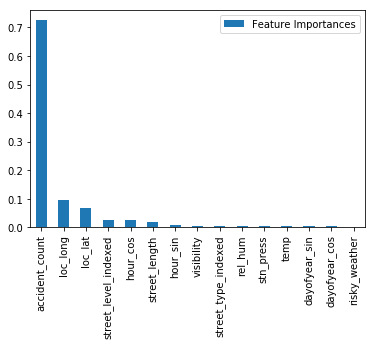
\includegraphics[height=7cm, keepaspectratio]{figures/feature_importances.png}}
\caption{Feature importances computed by the Balanced Random Forest}
\label{fig}
\end{figure}

\section{Results}
These results have been obtained by training the Balanced Random Forest algorithm on the whole dataset of positive samples, but with only half of the dataset of negative examples we have generated. Therefore the data imbalance is reduced to a factor of 8. To evaluate this model we used a test set containing the last two years of our dataset, the model is trained on the 4 previous years and use only data from these years. For example, the "count\_accident" feature contains only the count of accidents on road segments which occurred from 2012 to 2016.

We obtain an area under the precision-recall curve of 54\% and an area under the ROC curve of 89\% on the test dataset.
This results in the following precision and recall values depending on the chosen probability threshold:

\begin{figure}[htbp]
\centerline{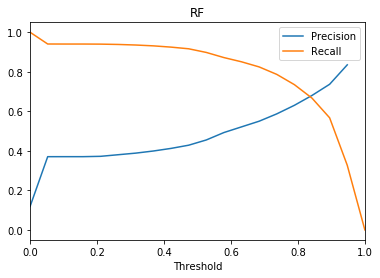
\includegraphics[height=6cm, keepaspectratio]{figures/pr.png}}
\caption{Precision and recall as a function of the probablity threshold}
\label{fig}
\end{figure}

As we can see, with a threshold set to 0.63, we can achieve a recall of 85\% with a precision of 0.29\%. With a threshold of 0.05, the model can actually detect almost all the accidents, 94\% of them, with a precision of 19\%, this corresponds to the high-risk roads and time.

\section{Discussion}
The overall results are good but mostly rely on the count of previous accidents on the road segment. This is not an issue for accident prediction, but it does not help to understand why these roads are particularly dangerous. Accident prediction is a very hard machine learning problem because even if the risk is very high for an accident to occur, and even if an accident almost occur, the by reacting quickly, the driver can manage to avoid it although the conditions were almost exactly the same as when an accident occurs. We would need information on the state of the drivers and the state of the vehicle to significantly improve performances. 

As opposed to what we would have expected, the Balance Random Forest did not obtained much better performances than the Random Forests with random undersampling. We believe this is caused by the fact that negative examples are not that different from each other and that the information they contains is well captured by a single random subsample. We can notice, that the Balance Random FOrest does not overfit as much as the Random Forest algorithm.

However, we believe these results can be improved even without this important feature by adding more spatial features. We can see that the most important variables are the features of the road segment. Therefore we believe providing more context information on where the road is located will greatly help. In another experiment, we have seen the population density and the distance to the closest billboard used as features successfully. However, even with more features and more data, it will be hard to reach very good performances because of the nature of the problem.

\subsection{Future work}
We believe better performances could be reached by adding more features from other datasets. For the city of Montreal, we identified two particularly interesting datasets: a dataset with the location and dates of construction work on roads, and a dataset with the population density. These datasets might not be as easily available for over areas, but for Montreal, it could improve performances. Also, the solar elevation and solar azimuth could easily be added without the need for another dataset. These features have been used successfully in road accident prediction in previous experiments.

\section*{Acknowledgment}

We acknowledge Compute Canada for giving us access to the cluster.

\bibliographystyle{IEEEtran}
\bibliography{biblio}

\end{document}
